\subsection{Evaluation}
\label{sec:evaluation}




The primary focus of this work lies in the
development
\LFCR as the first  CFL-reachability specification of \kcs{k} with
its own built-in call graph construction. In order to demonstrate its utility, we
have also developed \tool, the first \emph{precision-preserving} pre-analysis for accelerating \kcs{k} (\Cref{theorem:precisionpreserving}). In this section, we provide an experimental validation of this claim on \tool and compare it with two non-precision-preserving state-of-the-art pre-analyses, \selectx \cite{lu2021selective} and \zipper \cite{li2018precision}. Our
experimental results show that
\tool represents a new advance with better efficiency-precision trade-offs in a number of application scenarios highlighted below.


%This is made possible since \LFCR captures precisely all the value flows in a program (\Cref{thm:LFCR-correctness}).
\begin{comment}
Note that
 \selectx \cite{lu2021selective} is 
a \emph{non-precision-preserving} pre-analysis for accelerating \kcs{k}
as it is developed based on \manuLFC, which is
disconnected both
conceptually and algorithmically with the dynamic dispatch process done at a callsite
(as discussed in \Cref{subsec:condition}). 
Thus, there is not an apples-to-apples comparison between the two tools.
\end{comment}

\subsubsection{Experimental Setup}
\label{subsec:setup}


%\paragraph*{\bf Implementation} 

\begin{comment}
We have implemented \tool (\Cref{rule:toolrule})
in  \qilin \cite{he_et_al:LIPIcs.ECOOP.2022.30}, a pointer analysis
framework for Java developed on top of \soot \cite{vallee2010soot}. 
 As for
 \kcs{k} (i.e., Andersen's include-based formulation given in \Cref{rule:cfapta}), we use its implementation.
For a program,
we use \spark, a context-insensitive Andersen's pointer analysis  \cite{lhotak2003scaling} provided in \soot,
to build its PAG (including its call graph) needed by \tool.


For evaluation purposes,
we have followed a few common practices adopted in the  literature \cite{lu2019precision, lu2021selective, lu2021eagle, raghothaman2018user, tan2017efficient, He2021Turner, he2021context}. We use a reflection log generated by a dynamic reflection analysis tool, \textsc{TamiFlex} \cite{bodden2011taming} for resolving Java reflection. For native code, we use the method summaries provided in \qilin. String factory objects and exception-like objects are distinguished per dynamic type and analyzed context-insensitively.
\end{comment}

%\begin{comment}
%OLD ONE
%\paragraph*{\bf Implementation} 

We have implemented \kcs{k} (i.e., Andersen's inclusion-based formulation given in \Cref{rule:cfapta}) and \tool (\Cref{rule:toolrule})
in  \soot \cite{vallee2010soot} on top of its context-insensitive Andersen's pointer analysis, \spark \cite{lhotak2003scaling},
which is used for building the PAG of 
a program (including its call graph) for \tool. To compare \tool with \selectx and \zipper, we have reused their implementations provided in the \selectx artifact\footnote{\selectx artifact is available at \url{https://doi.org/10.5281/zenodo.4732680}}.
For evaluation purposes,
we have followed a few common practices adopted in the pointer analysis literature \cite{lu2019precision, lu2021selective, lu2021eagle, raghothaman2018user, tan2017efficient, He2021Turner, he2021context}. We use a reflection log generated by a dynamic reflection analysis tool, \textsc{TamiFlex} \cite{bodden2011taming} for resolving Java reflection. For native code, we use the method summaries provided in \soot. String factory objects and exception-like objects are distinguished per dynamic type and analyzed context-insensitively.


%\end{comment}

%\paragraph*{\bf Benchmarks} 

We have selected a set of  13 benchmarks from  the DaCapo benchmark suite (the latest version \texttt{6cf0380})
together with a large Java library (\texttt{JRE1.8.0\_31}).
%, which are frequently used in evaluating pointer analysis algorithms for Java \cite{smaragdakis2014introspective, kastrinis2013hybrid, tan2017efficient, li2018precision}. 
% For DaCapo, \texttt{luindex} is excluded as it is similar to \texttt{lusearch}. We have also excluded \texttt{jython} as its reflection log is overly conservative \cite{thiessen2017context}.
 We have excluded only \texttt{jython} as  all pointer analyses (evaluated in this section) except \spark cannot analyze this benchmark to completion under a time budget of 12 hours due to its overly conservative reflection log \cite{thiessen2017context}.

%\paragraph*{\bf Platform} 

We have carried out all our experiments on an Intel(R) Xeon(R) W-2245 3.90GHz machine with 512GB of RAM, running on Ubuntu 20.04.3 LTS (Focal Fossa). 



\begin{comment}
\begin{table}[htbp]
\centering
\setlength{\tabcolsep}{1.0ex}
\caption{The  precision and efficiency  of \kcs{k} and \pkcs{k}. For all metrics except  speedup, smaller is better.  \label{tab:main}}
 \vspace*{-1ex}
\scalebox{1.0}{
\addtolength{\tabcolsep}{1.4ex}
\def\arraystretch{.67}
\hspace{-3mm}
\small
\begin{tabular}{|c|l|r|r|r|r|}
	\hline
	 Program  & Metrics      &                           1CFA &                       \pkcs{1} &                             2CFA &                         \pkcs{2}\\ \hline \hline
	           & Time(secs)   &  16.8  &   4.7 \textcolor{blue}{(3.6x)} &   543.8  &   140.1 \textcolor{blue}{(3.9x)} \\
	           & \#Call Edges &                          55267 &                          55267 &                            54505 &                            54505 \\
	  avrora   & \#Poly Calls &                           1344 &                           1344 &                             1275 &                             1275 \\
	           & \#Fail Casts &                            931 &                            931 &                              890 &                              890 \\
	           & Avg PTS      &                          25.88 &                          25.88 &                            24.79 &                            24.79 \\ \hline
	           & Time(secs)   &  83.3  &  27.7 \textcolor{blue}{(3.0x)} &  1667.9  &   449.1 \textcolor{blue}{(3.7x)} \\
	           & \#Call Edges &                         151995 &                         151995 &                           147428 &                           147428 \\
	  batik    & \#Poly Calls &                           6637 &                           6637 &                             6397 &                             6397 \\
	           & \#Fail Casts &                           3709 &                           3709 &                             3485 &                             3485 \\
	           & Avg PTS      &                          71.68 &                          71.68 &                            66.65 &                            66.65 \\ \hline
	           & Time(secs)   &  48.9  &  23.1 \textcolor{blue}{(2.1x)} &  1158.0  &   332.2 \textcolor{blue}{(3.5x)} \\
	           & \#Call Edges &                          97960 &                          97960 &                            93662 &                            93662 \\
	 eclipse   & \#Poly Calls &                           3564 &                           3564 &                             3446 &                             3446 \\
	           & \#Fail Casts &                           2470 &                           2470 &                             2322 &                             2322 \\
	           & Avg PTS      &                          63.50 &                          63.50 &                            59.28 &                            59.28 \\ \hline
	           & Time(secs)   & 331.5  & 122.3 \textcolor{blue}{(2.7x)} &  5770.6  &  2368.4 \textcolor{blue}{(2.4x)} \\
	           & \#Call Edges &                         325547 &                         325547 &                           313954 &                           313954 \\
	   fop     & \#Poly Calls &                          16306 &                          16306 &                            15505 &                            15505 \\
	           & \#Fail Casts &                           8226 &                           8226 &                             7931 &                             7931 \\
	           & Avg PTS      &                         141.20 &                         141.20 &                           132.98 &                           132.98 \\ \hline
	           & Time(secs)   &  77.0  &  18.7 \textcolor{blue}{(4.1x)} &  6004.8  &  4335.9 \textcolor{blue}{(1.4x)} \\
	           & \#Call Edges &                         135775 &                         135775 &                           134234 &                           134234 \\
	    h2     & \#Poly Calls &                           5317 &                           5317 &                             5227 &                             5227 \\
	           & \#Fail Casts &                           2477 &                           2477 &                             2398 &                             2398 \\
	           & Avg PTS      &                          34.62 &                          34.62 &                            32.64 &                            32.64 \\ \hline
	           & Time(secs)   &  40.4  &  22.7 \textcolor{blue}{(1.8x)} &   749.7  &   227.5 \textcolor{blue}{(3.3x)} \\
	           & \#Call Edges &                          79431 &                          79431 &                            78190 &                            78190 \\
	 luindex   & \#Poly Calls &                           2615 &                           2615 &                             2537 &                             2537 \\
	           & \#Fail Casts &                           1359 &                           1359 &                             1286 &                             1286 \\
	           & Avg PTS      &                          24.76 &                          24.76 &                            23.04 &                            23.04 \\ \hline
	           & Time(secs)   &  12.6  &   3.6 \textcolor{blue}{(3.5x)} &   444.7  &   132.8 \textcolor{blue}{(3.3x)} \\
	           & \#Call Edges &                          43117 &                          43117 &                            42412 &                            42412 \\
	 lusearch  & \#Poly Calls &                           1254 &                           1254 &                             1189 &                             1189 \\
	           & \#Fail Casts &                            702 &                            702 &                              660 &                              660 \\
	           & Avg PTS      &                          20.74 &                          20.74 &                            19.73 &                            19.73 \\ \hline
	           & Time(secs)   & 112.9  &  42.8 \textcolor{blue}{(2.6x)} & 16270.6  & 14135.0 \textcolor{blue}{(1.2x)} \\
	           & \#Call Edges &                         153150 &                         153150 &                           152090 &                           152090 \\
	   pmd     & \#Poly Calls &                           6707 &                           6707 &                             6656 &                             6656 \\
	           & \#Fail Casts &                           4321 &                           4321 &                             4233 &                             4233 \\
	           & Avg PTS      &                          68.77 &                          68.77 &                            67.48 &                            67.48 \\ \hline
	           & Time(secs)   &  27.0  &   7.5 \textcolor{blue}{(3.6x)} &   600.0  &   166.8 \textcolor{blue}{(3.6x)} \\
	           & \#Call Edges &                          74198 &                          74198 &                            73392 &                            73392 \\
	 sunflow   & \#Poly Calls &                           2524 &                           2524 &                             2454 &                             2454 \\
	           & \#Fail Casts &                           1771 &                           1771 &                             1649 &                             1649 \\
	           & Avg PTS      &                          33.63 &                          33.63 &                            31.35 &                            31.35 \\ \hline
	           & Time(secs)   &  19.1  &   5.7 \textcolor{blue}{(3.4x)} &   682.9  &   148.6 \textcolor{blue}{(4.6x)} \\
	           & \#Call Edges &                          57933 &                          57933 &                            57073 &                            57073 \\
	  tomcat   & \#Poly Calls &                           1622 &                           1622 &                             1554 &                             1554 \\
	           & \#Fail Casts &                            959 &                            959 &                              874 &                              874 \\
	           & Avg PTS      &                          25.37 &                          25.37 &                            24.03 &                            24.03 \\ \hline
	           & Time(secs)   &  25.1  &   7.7 \textcolor{blue}{(3.3x)} &   599.0  &   170.4 \textcolor{blue}{(3.5x)} \\
	           & \#Call Edges &                          67742 &                          67742 &                            66814 &                            66814 \\
	tradebeans & \#Poly Calls &                           2049 &                           2049 &                             2003 &                             2003 \\
	           & \#Fail Casts &                           1132 &                           1132 &                             1054 &                             1054 \\
	           & Avg PTS      &                          31.80 &                          31.80 &                            29.96 &                            29.96 \\ \hline
	           & Time(secs)   &  24.6  &   7.7 \textcolor{blue}{(3.2x)} &   652.9  &   169.7 \textcolor{blue}{(3.8x)} \\
	           & \#Call Edges &                          67742 &                          67742 &                            66814 &                            66814 \\
	tradesoap  & \#Poly Calls &                           2049 &                           2049 &                             2003 &                             2003 \\
	           & \#Fail Casts &                           1132 &                           1132 &                             1054 &                             1054 \\
	           & Avg PTS      &                          31.80 &                          31.80 &                            29.96 &                            29.96 \\ \hline
	           & Time(secs)   &  28.2  &   7.1 \textcolor{blue}{(4.0x)} &   808.8  &   160.2 \textcolor{blue}{(5.0x)} \\
	           & \#Call Edges &                          67132 &                          67132 &                            66360 &                            66360 \\
	  xalan    & \#Poly Calls &                           2755 &                           2755 &                             2692 &                             2692 \\
	           & \#Fail Casts &                           1473 &                           1473 &                             1419 &                             1419 \\
	           & Avg PTS      &                          29.41 &                          29.41 &                            28.30 &                            28.30 \\ \hline\hline
\end{tabular}
	}
\end{table}
\end{comment}

\begin{table}[]
    \centering
\setlength{\tabcolsep}{1.0ex}
\caption{The  precision and efficiency  of \kcs{k}, \pkcs{k} (\kcs{k} accelerated by \tool), \skcs{k} (\kcs{k} accelerated by \selectx), and \zkcs{k} (\kcs{k} accelerated by \zipper). The results for \spark are also included. 
For each main analysis in $A\in \{
\pkcs{k},
\skcs{k},
\zkcs{k}\}$, the analysis times
 are given as $x (y)$, where $x$ is the
 analysis time of $A$ and $y$ is
 the corresponding pre-analysis time (in seconds). For all metrics, smaller is better.  \label{tab:main}}
 \vspace*{-1ex}
\scalebox{0.84}{
\addtolength{\tabcolsep}{-0.65ex}
\def\arraystretch{.85}
\hspace{-3mm}
\small

\begin{tabular}{|c|l|r||r|>{\columncolor{pink!35}}r|>{\columncolor{lightgray!75}}r|>{\columncolor{orange!15}}r||r|>{\columncolor{pink!35}}r|>{\columncolor{lightgray!75}}r|>{\columncolor{orange!15}}r|}
\hline
Program&Metrics&\textsc{Spark}&1CFA&$P$-1CFA&$S$-1CFA&$Z$-1CFA&2CFA&$P$-2CFA&$S$-2CFA&$Z$-2CFA\\
\hline
&Time(secs)&6.6&18.0&4.7 (1.2)&3.1 (21.5)&2.8 (4)&577.1&142.5 (1.2)&16.8 (21.6)&11.2 (4)\\
&\#Call Edges&57509&55267&55267&55267&55403&54505&54505&54506&54662\\
avrora&\#Fail Casts&1197&931&931&931&965&890&890&895&942\\
&\#Alias Pairs&22327&13700&13700&13700&13703&13268&13268&13280&13547\\
&Avg PTS&36.19&25.87&25.87&25.87&26.48&24.78&24.78&24.80&25.47\\
\hline
&Time(secs)&30.9&81.0&28.0 (4.7)&25.3 (169.5)&23.1 (243)&1473.9&466.5 (4.8)&271.1 (174.4)&276.5 (234)\\
&\#Call Edges&171409&151995&151995&151997&152025&147428&147428&147430&150549\\
batik&\#Fail Casts&4573&3709&3709&3709&3713&3485&3485&3490&3620\\
&\#Alias Pairs&68130&38005&38005&38005&38012&32288&32288&32300&33295\\
&Avg PTS&114.43&71.67&71.67&71.67&71.71&66.65&66.65&66.65&68.21\\
\hline
&Time(secs)&14.8&48.7&23.3 (2.0)&20.1 (54.6)&19.7 (14)&1221.1&331.0 (2.0)&171.8 (56.8)&143.9 (14)\\
&\#Call Edges&110089&97960&97960&98000&98052&93662&93662&93703&93746\\
eclipse&\#Fail Casts&2896&2470&2470&2471&2474&2322&2322&2328&2337\\
&\#Alias Pairs&107389&58489&58489&58500&58504&51404&51404&51427&51716\\
&Avg PTS&101.12&63.49&63.49&63.47&63.80&59.28&59.28&59.26&59.64\\
\hline
&Time(secs)&76.0&318.8&123.1 (10.6)&113.1 (603.8)&104.0 (355)&6019.6&2399.6 (10.8)&1901.7 (604.5)&1405.1 (354)\\
&\#Call Edges&358738&325547&325547&325551&325591&313954&313954&313958&321008\\
fop&\#Fail Casts&9057&8226&8226&8228&8239&7931&7931&7938&8084\\
&\#Alias Pairs&323628&277047&277047&277047&277065&267389&267389&267401&268943\\
&Avg PTS&233.48&141.19&141.19&141.19&141.25&132.98&132.98&132.98&135.43\\
\hline
&Time(secs)&16.1&75.7&18.5 (2.9)&15.8 (74.1)&14.3 (40)&6406.8&4164.6 (2.8)&3807.8 (74.4)&3127.4 (39)\\
&\#Call Edges&144711&135775&135775&135782&135806&134234&134234&134241&134274\\
h2&\#Fail Casts&2880&2477&2477&2477&2482&2398&2398&2404&2433\\
&\#Alias Pairs&77978&39209&39209&39209&39236&33331&33331&33351&33632\\
&Avg PTS&72.61&34.61&34.61&34.61&34.68&32.63&32.63&32.64&33.20\\
\hline
&Time(secs)&18.5&41.0&24.0 (1.9)&22.6 (48.1)&20.1 (8)&829.1&232.3 (1.9)&109.0 (48.2)&82.3 (8)\\
&\#Call Edges&85850&79431&79431&79431&79602&78190&78190&78190&78404\\
luindex&\#Fail Casts&1726&1359&1359&1360&1376&1286&1286&1292&1314\\
&\#Alias Pairs&50530&32905&32905&32905&32908&31795&31795&31807&32083\\
&Avg PTS&53.10&24.75&24.75&24.75&24.87&23.04&23.04&23.04&23.15\\
\hline
&Time(secs)&5.3&12.6&3.5 (1.0)&2.3 (13.9)&1.9 (3)&414.0&129.3 (1.0)&9.6 (13.9)&7.1 (3)\\
&\#Call Edges&45285&43117&43117&43117&43198&42412&42412&42412&42516\\
lusearch&\#Fail Casts&955&702&702&702&719&660&660&665&696\\
&\#Alias Pairs&20382&11693&11693&11693&11696&11263&11263&11275&11542\\
&Avg PTS&31.38&20.73&20.73&20.74&20.85&19.73&19.73&19.75&19.94\\
\hline
&Time(secs)&20.3&109.5&42.6 (3.0)&37.2 (139.1)&35.9 (25)&16006.8&13715.8 (3.0)&13671.4 (139.1)&9356.3 (25)\\
&\#Call Edges&159395&153150&153150&153150&153387&152090&152090&152090&152242\\
pmd&\#Fail Casts&4702&4321&4321&4321&4325&4233&4233&4238&4263\\
&\#Alias Pairs&114914&95977&95977&95977&95979&93083&93083&93095&93353\\
&Avg PTS&90.97&68.76&68.76&68.76&68.79&67.48&67.48&67.49&67.58\\
\hline
&Time(secs)&9.9&25.9&7.4 (1.8)&5.5 (46.4)&5.3 (9)&643.1&165.1 (1.7)&33.0 (45.9)&27.7 (9)\\
&\#Call Edges&77346&74198&74198&74200&74241&73392&73392&73394&73685\\
sunflow&\#Fail Casts&2192&1771&1771&1773&1776&1649&1649&1656&1684\\
&\#Alias Pairs&36952&21670&21670&21670&21678&20703&20703&20715&21041\\
&Avg PTS&51.31&33.62&33.62&33.62&33.69&31.34&31.34&31.36&31.79\\
\hline
&Time(secs)&7.4&18.9&5.8 (1.3)&4.0 (20.8)&3.7 (4)&632.9&148.7 (1.3)&16.1 (20.8)&11.7 (4)\\
&\#Call Edges&60649&57933&57933&57933&58024&57073&57073&57073&57369\\
tomcat&\#Fail Casts&1264&959&959&960&963&874&874&880&910\\
&\#Alias Pairs&30775&24504&24504&24504&24507&22202&22202&22214&22482\\
&Avg PTS&39.88&25.37&25.37&25.37&25.51&24.03&24.03&24.04&24.62\\
\hline
&Time(secs)&8.7&25.9&7.6 (1.5)&5.6 (41.7)&5.2 (9)&737.4&166.5 (1.5)&30.2 (43.4)&18.2 (9)\\
&\#Call Edges&70911&67742&67742&67742&67858&66814&66814&67018&67207\\
tradebeans&\#Fail Casts&1523&1132&1132&1132&1135&1054&1054&1059&1068\\
&\#Alias Pairs&36256&27175&27175&27175&27178&25683&25683&25695&25950\\
&Avg PTS&47.67&31.80&31.80&31.80&31.87&29.95&29.95&29.98&30.18\\
\hline
&Time(secs)&8.4&24.8&7.7 (1.6)&5.8 (46.8)&5.2 (9)&703.0&162.8 (1.5)&29.9 (49.4)&17.9 (9)\\
&\#Call Edges&70911&67742&67742&67742&67858&66814&66814&67018&67207\\
tradesoap&\#Fail Casts&1523&1132&1132&1132&1135&1054&1054&1059&1068\\
&\#Alias Pairs&36256&27175&27175&27175&27178&25683&25683&25695&25950\\
&Avg PTS&47.67&31.80&31.80&31.80&31.87&29.95&29.95&29.98&30.18\\
\hline
&Time(secs)&8.5&27.3&7.4 (1.4)&5.5 (42.6)&5.0 (16)&702.8&162.3 (1.6)&34.2 (42.3)&26.0 (16)\\
&\#Call Edges&69608&67132&67132&67132&67210&66360&66360&66360&66448\\
xalan&\#Fail Casts&1807&1473&1473&1473&1477&1419&1419&1424&1441\\
&\#Alias Pairs&42119&28280&28280&28280&28283&27259&27259&27271&27539\\
&Avg PTS&45.29&29.41&29.41&29.41&29.47&28.29&28.29&28.30&28.41\\
\hline
\hline
\end{tabular}

}
\end{table}


\subsubsection{Results} 

\Cref{tab:main} contains the results for \kcs{k}, \pkcs{k} (i.e., \kcs{k} accelerated by \tool),  \skcs{k} (i.e., \kcs{k} accelerated by \selectx), and \zkcs{k} (i.e., \kcs{k} accelerated by \zipper), where $k \in \{1, 2\}$.
The results for \spark are also included for comparison
purposes.
\begin{comment}
\Cref{tab:pretime} gives the analysis times of \spark and \tool.
\end{comment}
Note that for $k\geqslant 3$,
\kcs{k} is unscalable for all the 13 programs 
under a time budget
of 12 hours and thus has never been considered
in the pointer analysis literature 
\cite{lu2021selective, raghothaman2018user,
li2018precision, li2020principled,tan2017efficient, smaragdakis2011pick,jeon2018precise,thiessen2017context}.

\begin{comment}


Note that for $k\geqslant 3$, \kcs{k} currently
cannot  analyze scalably any of the 13 benchmarks considered  under a time budget
of 12 hours on our platform. This is also true for other implementations of \kcs{k}, such
as those in \doop~\cite{bravenboer2009strictly}
and
 \wala~\cite{WALA2022}.
\end{comment}


%Below we will compare \pkcs{k} with \kcs{k} (as the baseline) in terms of precision  and efficiency. We will also discuss the effectiveness of \tool (as a pre-analysis).



\paragraph*{Precision}
\label{subsec:precision}

We measure the precision of a pointer analysis by considering four commonly used metrics \cite{smaragdakis2011pick, feng2015bottom, tan2017efficient, lu2019precision, li2018precision, He2021Turner}:
(1) ``\#Call Edges'': the number of call graph edges discovered,  
%(2) ``\#Poly Calls'': the number of polymorphic calls discovered, 
(2) ``\#Fail Casts'': the number of type casts that may fail, 
(3) ``\#Alias Pairs'': the number of base variable pairs of stores and loads  that are queried to be may-alias with trivial must aliases (e.g., due to  direct assignments) being excluded \cite{feng2015bottom},
and (4) ``Avg PTS'': the average number of objects pointed by a variable  by considering only the local variables in the Java methods (being analyzed).
For each of the four precision metrics, smaller is better.

For each  metric $M$, $M_{PTA}$ denotes the result obtained by $PTA$, where $PTA$ denotes any pointer analysis in \{\spark, \kcs{k}, \pkcs{k}, \skcs{k}, \zkcs{k}\}. Let $\Akcs{k}\in \{\pkcs{k}, \skcs{k}, \zkcs{k}\}$ be one of the three
variants of \kcs{k}
such that $\Akcs{k}$ is no less precise than \spark but
no more precise than \kcs{k}. We define the precision loss of $\Akcs{k}$ with respect to $\kcs{k}$ on metric $M$ as:
\begin{equation}
\label{eq:precisionloss}
    \Delta_{\Akcs{k}}^{M} = \frac{(M_{\spark} - M_{\kcs{k}}) - (M_{\spark} - M_{\Akcs{k}})}{M_{\spark} - M_{\kcs{k}}} = \frac{M_{\Akcs{k}} - M_{\kcs{k}}}{M_{\spark} - M_{\kcs{k}}}
\end{equation}
The precision improvement going from \spark to $\kcs{k}$ (considered as the
baseline) is regarded as 100\%. If $M_{\Akcs{k}} = M_{\kcs{k}}$ (i.e., $\Akcs{k}$ is equally precise as $\kcs{k}$), then
$\Delta_{\Akcs{k}}^{M}=0\%$, implying that
$\Akcs{k}$ loses no precision at all. On the other hand, if $M_{\Akcs{k}} = M_{\spark}$ (i.e.,
$\Akcs{k}$ degenerates into \spark), then
$\Delta_{\Akcs{k}}^{M}=100\%$, implying that
$\Akcs{k}$ loses all the precision gained by $\kcs{k}$. 
%In this paper, $Baseline$ is \kcs{k} and $A$ can be any pointer analysis from \{\pkcs{k}, \skcs{k}, \zkcs{k}\}. 

For all the 13 benchmarks considered,
\pkcs{k} is always precision-preserving (i.e., for each precision metric $M$ considered, $\Delta_{\pkcs{k}}^{M} = 0\%$ always holds)  as proved in
\Cref{theorem:precisionpreserving} and validated further in \Cref{tab:main} with
\pkcs{k} producing exactly the same points-to results as \kcs{k}.

\Cref{fig:precisionlosses} plots the precision loss of \skcs{2} and \zkcs{2}.
As shown in \Cref{fig:selectxprecisionloss},
 \skcs{2} suffers from only a small loss of precision (0.8\%, 1.2\%, 0.1\% and 0.1\% for ``\#Call Edges'', ``\#Fail Casts'', ``\#Alias Pairs'' and ``Avg PTS'', respectively, on average) as \selectx exploits \manuLFC \cite{sridharan2006refinement} for making its context-sensitivity selections. We will  introduce two examples below to explain the relatively large precision loss observed in \texttt{tradebeans}, \texttt{tradesoap}  and
 \texttt{eclipse}. 
 On the  other hand, as shown in \Cref{fig:zipperprecisionloss},
 \zkcs{2}  suffers from a higher  precision loss as \zipper exploits pattern-based 
 heuristics to make its context-sensitivity selections. On average, its precision loss percentages for ``\#Call Edges'', ``\#Fail Casts'', ``\#Alias Pairs'', and ``Avg PTS'' are 6.2\%, 8.1\%, 2.2\%, and 2.0\%, respectively.

\begin{comment}
By \Cref{theorem:precisionpreserving}, \tool is precision-preserving as it reasons about CFL-reachability to select a superset of precision-critical variables to be analyzed context-sensitively. The evaluation (Columns 5 and 8 in \Cref{tab:main}) confirms \Cref{theorem:precisionpreserving} by shown that all the four precision-related metrics are exactly same as their baseline analyses.
\end{comment}

\begin{comment}

\tooll preserves the precision for 10 out of 13 programs except that \texttt{pmd} and \texttt{findbugs}. The slightly precision loss is caused by a rarely occurring subtle case, \textit{the null-receiver problem}, as will be illustrated in \Cref{fig:toollPrecisionLossExample}.

In \Cref{fig:toollPrecisionLossExample}, a total of 4 classes, i.e., \texttt{A}, \texttt{B}, \texttt{C}, and
\texttt{D}, are defined. Class \texttt{D} is a subclass of \texttt{C}. Class \texttt{A} defines a method \texttt{foo()}, in which the method 
\texttt{bar()} created in Class \texttt{B} is invoked on variable \texttt{b}, which is a dereference of \texttt{this.f} (line 3). In \texttt{main()}, \texttt{foo()} is invoked twice at two different callsites (lines~20-21) with \commentfont{A1} and \commentfont{A2} as their corresponding receiver objects respectively. 

In \kcs{1}, \texttt{foo()} will be analyzed under two different contexts, say [$l_{20}$] and [$l_{21}$]. \texttt{bar()} is only invoked at line 5 thus only have one calling context [$l_{5}$]. In [$l_{20}$], we have $\pointsto(c, [l_{20}]) = \{$\commentfont{C}$\}$, $\pointsto(\mathtt{this}, [l_{20}]) = \{$\commentfont{A1}$\}$, 
and $\pointsto(b, [l_{20}]) \linebreak = \pointsto($\commentfont{A1}$.f, \emptyctx) = \emptyset$. Since the points-to set of \texttt{b} under $[l_{20}]$ is empty, the points-to set of \texttt{c} under the same context will not be propagated to \texttt{p}. In [$l_{21}$], similarly, we have $\pointsto(c, [l_{21}]) = \{$\commentfont{D}$\}$, $\pointsto(\mathtt{this}, [l_{21}]) = \{$\commentfont{A2}$\}$, 
and $\pointsto(b, [l_{21}]) \linebreak = \pointsto($\commentfont{A2}.f$, \emptyctx) = \  \{$\commentfont{B2}$\}$. This time, the dispatching algorithm resolves the call at line 5 to \texttt{bar()} and propagate the values of \texttt{c} under [$l_{21}$] to \texttt{p}, thus we have $\pointsto(p, [l_5]) = \{$\commentfont{D}$\}$ and context-insensitively $\cipointsto{p} = \{$\commentfont{D}$\}$. Finally, at line 9, \kcs{1} does not report a may-fail-cast error as \texttt{p} only has only type, i.e., \texttt{D}. 

In \lkcs{1}, \tooll will identify \lstinline{b.bar(c)} (line 5) as a monomorphic call according to the context-insensitive points-to information obtained from \spark \cite{lhotak2003scaling}. Thus, \tooll does not find dispatching type for \lstinline{b.bar(c)} at line 5 but directly handles inter-procedural assign edges as usual \cite{lu2021selective, sridharan2005demand, sridharan2006refinement}. As a result, \tooll mis-identifies \texttt{b}, \texttt{c},
and \texttt{this} in \texttt{foo()} as precision-uncritical variables and analyzed context-insensitively during \lkcs{1}. Then, we have 
$\pointsto(\mathtt{this}, \emptyctx) = \{$\commentfont{A2}$\}$, 
$\pointsto(b, \emptyctx) = \pointsto($\commentfont{A2}.f$, \emptyctx) = \  \{$\commentfont{B2}$\}$, and $\pointsto(p, \emptyctx) = \pointsto(c, \emptyctx) = \{$\commentfont{C}, \commentfont{D}$\}$. Note, \texttt{p} and \texttt{d} in \texttt{bar()} analyzed context-insensitively by \tooll are indeed precision-uncritical. Finally, \commentfont{D} in $\cipointsto{p}$ is spurious, resulting \tooll to report a cast blame in line 9.

As confirmed in \Cref{tab:main}, such a precision loss case rarely happens in practice, making \tooll almost precision-preserving for most of programs.

\begin{figure}[htbp]
	\centering
\begin{subfigure}{\linewidth}
    \begin{subfigure}{.525\linewidth}
\begin{lstlisting}[basicstyle=\small]
class A { B f;
  void foo(C c) {
    B b = this.f;
    if (!b) return;
    b.bar(c);
}}
class B {
  void bar(C p) {
    D d = (D) p; //fail?
  }
}
\end{lstlisting}
    \end{subfigure}
    \begin{subfigure}{.465\linewidth}
\begin{lstlisting}[language=java, firstnumber=12, basicstyle=\small]
class C {}
class D extends C {}
void main() {
  B b2 = new B(); // B2
  A a1 = new A(); // A1
  A a2 = new A(); // A2
  // a1.f = null;
  a2.f = b2;
  a1.foo(new C()); // C
  a2.foo(new D()); // D
}
\end{lstlisting}
    \end{subfigure}
\end{subfigure}
	\caption{A motivating example for illustrating precision loss of \tooll. Variables in \texttt{foo()} analyzed context-insensitively by \lkcs{1} falsely reports a cast blame in line 9.}
	\label{fig:toollPrecisionLossExample}
\end{figure}
\end{comment}

\begin{figure}[t]
\centering
\begin{subfigure}[b]{\textwidth}
     \centering
     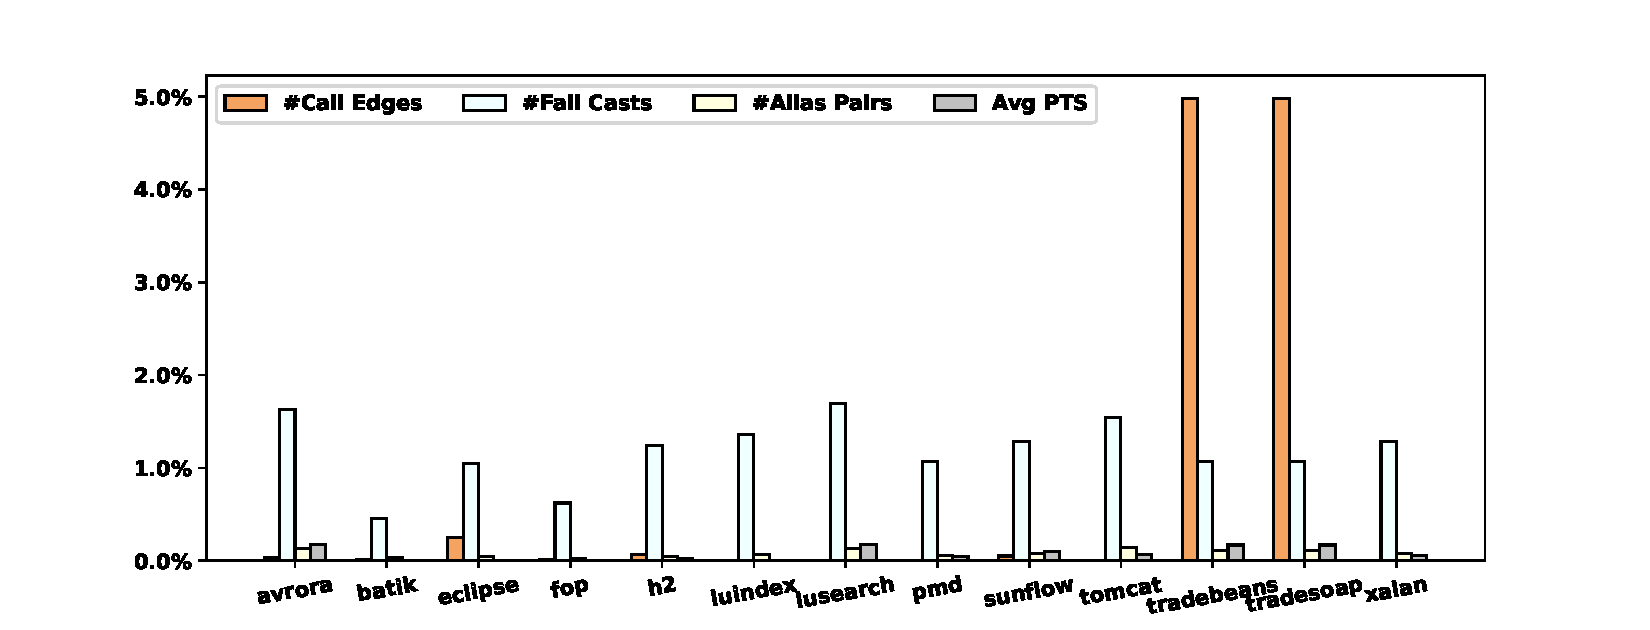
\includegraphics[width=\textwidth]{precisionlossSelectx.pdf}
     \caption{Precision loss of \skcs{2}}
     \label{fig:selectxprecisionloss}
 \end{subfigure}
 \hfill
 \begin{subfigure}[b]{\textwidth}
     \centering
     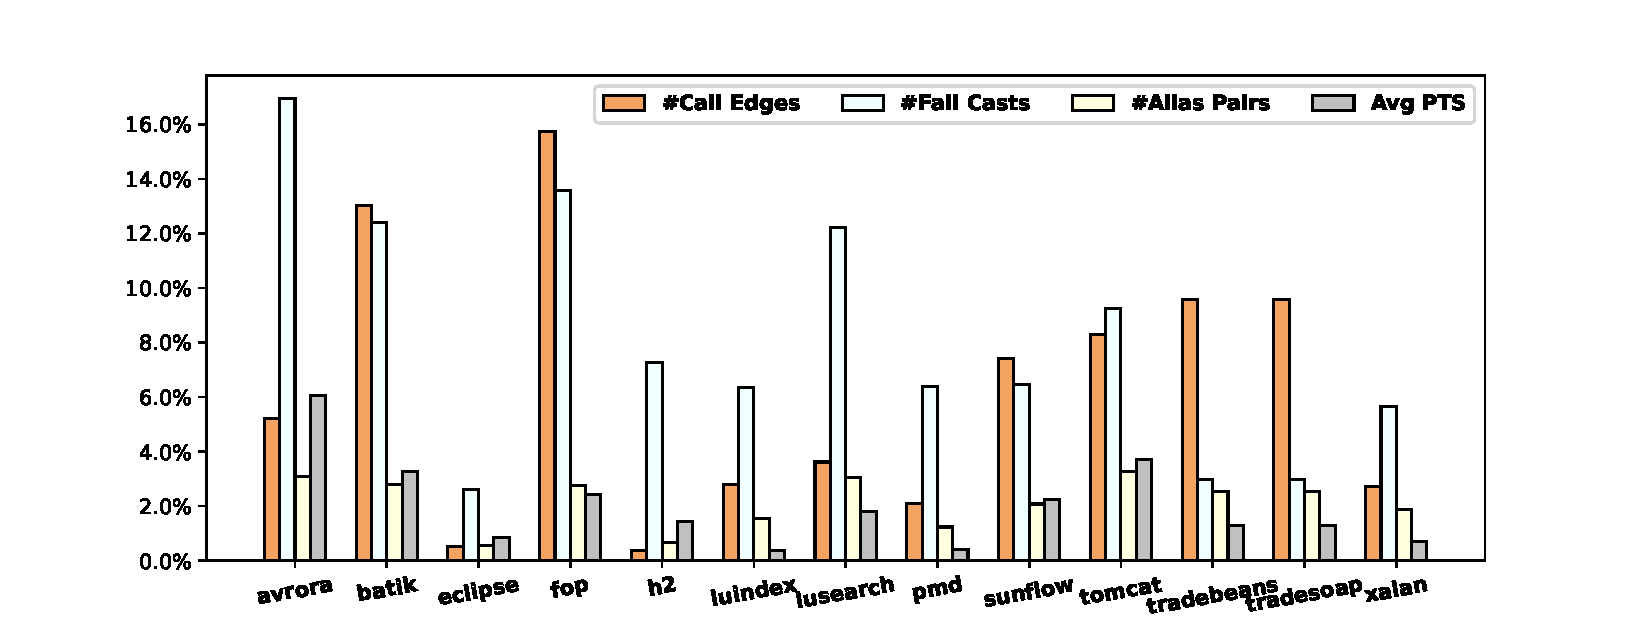
\includegraphics[width=\textwidth]{precisionlossZipper.pdf}
     \caption{Precision loss of \zkcs{2}}
     \label{fig:zipperprecisionloss}
\end{subfigure}
\caption{The precision loss of \skcs{2} and \zkcs{2} (computed according to \Cref{eq:precisionloss}). 
%relative to \kcs{k} and also \pkcs{k} (since \pkcs{k} is always precision-preserving as guaranteed by \Cref{theorem:precisionpreserving})  by using the results obtained from \Cref{tab:main} for all the 13 programs where $k = 2$.
\label{fig:precisionlosses}}
\end{figure}

\Cref{fig:treemap} gives an example for illustrating why \skcs{2} loses 
precision in \texttt{tradebeans} and \texttt{tradesoap}. Unlike 
\pkcs{2},
\skcs{2}
fails to
identify the call in line 15 as a monomorphic call to 
\texttt{toString()} defined in \texttt{java.lang.String}. 
This example includes three classes with \texttt{TreeMap} and  \linebreak
\texttt{CaseInsensitiveComparator} abstracted from \texttt{JDK8} and 
\texttt{StringComparator} abstracted from  \linebreak \texttt{tradebeans}. 
In \texttt{main()}, two \texttt{TreeMap} objects are created and used as the receiver objects to 
invoke \texttt{put()} 
with an integer object and a string object as its first argument, 
respectively (lines 26-27). When \texttt{put()} is invoked on each
\texttt{TreeMap} object,
a virtual call \texttt{compare()} is invoked on the 
 \texttt{comparator} object stored in the \texttt{TreeMap} object. 
When \kcs{2} is applied, \texttt{put()} will be analyzed under two  calling contexts, 
$[\mathtt{c1}]$ and $[\mathtt{c2}]$.
%As a result, \texttt{toString()} in line 15 has two different calling contexts, $[\mathtt{c3}, \mathtt{c1}]$ and  $[\mathtt{c3}, \mathtt{c2}]$.
Under $[\mathtt{c1}]$,
\texttt{cmp} points to  \commentfont{O1} and  \texttt{k} points to \commentfont{O5}, 
so that \texttt{compare()} defined in line 10 is identified to be called under 
$[\mathtt{c3}, \mathtt{c1}]$
in line 6. Under $[\mathtt{c2}]$,  \texttt{cmp} 
points to \commentfont{O2} and  \texttt{k} points to \commentfont{O6},
so that \texttt{compare()} defined in line 14 is called under
$[\mathtt{c3}, \mathtt{c2}]$
in line 6, in which case, 
 \texttt{o1} points to \commentfont{O6} uniquely in line 14. 
 As a result, the virtual call made in line 15 invokes only the \texttt{toString()} method defined in \texttt{java.lang.String}. 
 \selectx relies on  \manuLFC~\cite{sridharan2006refinement}
 to make its
context-sensitivity selections and will identify \texttt{cmp} and \texttt{k} in \texttt{put()} to be context-insensitive since \selconThree in \Cref{eqn:cflcscondition} is not satisfied with respect to \manuLFC.  When
\skcs{2} is applied,
 %\texttt{cmp} will point to both \texttt{O1} and \texttt{O2},
% and \texttt{k} and 
\texttt{o1} is found to
point to both \commentfont{O5} and \commentfont{O6}  conservatively
even under  $[\mathtt{c3}, \mathtt{c2}]$, making the call in line 15 polymorphic 
incorrectly
(with its two call targets being \texttt{toString()} in 
\texttt{java.lang.String} and \texttt{toString()} in 
\texttt{java.lang.Integer}). In contrast, \tool makes its context-sensitivity selections based on  \LFCR, concluding that \texttt{cmp} and \texttt{k} in \texttt{put()} should be context-sensitive since \selconThree in \Cref{eqn:cflcscondition} is satisfied with respect to \LFCR. 
%In \LFCR, whenever a value flows to a virtual call (e.g., line 6), the \LF will enforce the value flow to find a points-to object of the receiver variable (e.g., \texttt{cmp}), making the flow out of the method (i.e., satisfying  \selconThree ). 
 When \pkcs{2} is applied,
 \texttt{o1} is found to
point to  \commentfont{O6} uniquely
 under context $[\mathtt{c3}, \mathtt{c2}]$, making the call in line 15  monomorphic
 correctly. When analyzing \texttt{tradebeans} and \texttt{tradesoap}, 
 \skcs{2} suffers from a precision loss of about 5\% for ``\#Call Edges'' this way, which can be undesirable
 for many precision-critical client analyses such as software security analysis.

\Cref{fig:eclipsePrecisionLoss} gives another example abstracted from \texttt{eclipse} and \texttt{JDK8} to further illustrate why \skcs{2} can lose precision. The
situation for \skcs{1} is similar.
In  line 23 (26) of \texttt{main()}, we call \texttt{execute()} with \commentfont{O2} (\commentfont{O5}) as the receiver object and \commentfont{O4} (\commentfont{O6}) as its argument. As \selectx will
select
all the variables in \texttt{execute()} and \texttt{reject()}  to be context-insensitive (for the similar reasons discussed in the previous example), 
\skcs{2} will conclude that 
% \texttt{r} points to \commentfont{O4} and \commentfont{O6},
$\pointsto(\texttt{r}, \emptyctx) = \{\langle \commentfont{O4}, \emptyctx\rangle, \langle\commentfont{O6}, \emptyctx\rangle\}$, 
making the call
to \texttt{run()} in line 6 polymorphic. In contrast, \tool will select
all the variables in \texttt{execute()} and \texttt{reject()} to be context-sensitive.  When \pkcs{2} is applied,
\texttt{reject()} has two calling contexts,  $[\mathtt{c3}, \mathtt{c1}]$ and $[\mathtt{c3}, \mathtt{c2}]$. Under  $[\mathtt{c3}, \mathtt{c1}]$, we find that 
% $\texttt{this}^\texttt{reject}$ points to \commentfont{O2}, 
$\pointsto(\texttt{this}^\texttt{reject}, [\mathtt{c3}, \mathtt{c1}]) = \{\langle \commentfont{O2}, \emptyctx \rangle\}$, 
%\commentfont{O2}.\texttt{handler} points to \commentfont{O1},
$\pointsto(\commentfont{O2}.\texttt{handler}, \emptyctx) = \{\langle \commentfont{O1}, \emptyctx \rangle\}$, 
and $\pointsto(\texttt{r}, [\mathtt{c4}, \mathtt{c3}]) = \pointsto(\texttt{p}, [\mathtt{c3}, \mathtt{c1}]) = \{\langle \commentfont{O4}, \emptyctx \rangle\}$. 
% and \texttt{r} and \texttt{p} point to \commentfont{O4}.
Under  $[\mathtt{c3}, \mathtt{c2}]$, we find
that $\pointsto(\texttt{this}^\texttt{reject}, [\mathtt{c3}, \mathtt{c2}]) = \{\langle \commentfont{O5}, \emptyctx \rangle\}$ and $\pointsto(\commentfont{O5}.\texttt{handler}, \emptyctx) = \emptyset$, and in addition, whatever \texttt{p}
points to cannot be passed to  \texttt{r}. By combining these two cases, 
\pkcs{2} concludes that \texttt{r} only points to \commentfont{O4},
% $\cipointsto{\texttt{r}} = \{\commentfont{O4}\}$, 
and consequently, the call to \texttt{run()} in line 6
is  monomorphic. When analyzing \texttt{eclipse}, \skcs{2}
introduces dozens of such spurious call edges.
%since method
%\texttt{run()} defined in line 17 invokes many other methods in its body. 

\begin{figure}[t]
\begin{center}
\begin{mdframed}[
align=center,
usetwoside=false,
 rightmargin=0.5cm,
innerleftmargin=1.0ex,
innertopmargin=0.2ex,
innerbottommargin=0.2ex
]
\begin{lstlisting}[language=java]
class TreeMap {
  Comparator comparator;
  TreeMap(Comparator cmp1) { this.comparator = cmp1; }
  void put(Object k, Object v) {
    Comparator cmp = this.comparator;
    int i = cmp.compare(k, ...); // c3
}}
// in java.lang.String 
class CaseInsensitiveComparator implements Comparator {
  int compare(String p1, String p2) { return 0; }
}
// in org.apache.geronimo.main
class StringComparator implements Comparator {
  int compare(Object o1, Object o2) {
    String s1 = o1.toString(); // #Call Edges?
    return s1.compareTo(o2.toString()); 
}}
void main() {
  Comparator cmp1 = new CaseInsensitiveComparator(); // O1
  Comparator cmp2 = new StringComparator(); // O2
  TreeMap map1 = new TreeMap(cmp1); // O3
  TreeMap map2 = new TreeMap(cmp2); // O4
  Integer x = new Integer(1); // O5
  String y = new String(); // O6
  z = new String(); // O7
  map1.put(x, z); // c1
  map2.put(y, z); // c2
}
\end{lstlisting}
\end{mdframed}
\end{center}
\caption{An example abstracted from \texttt{tradebeans} and \texttt{JDK8} to illustrate why \selectx  is not precision-preserving
(by applying \manuLFC to determine
precision-critical variables/objects in  a program). 
\label{fig:treemap}}
\end{figure}


\begin{figure}[h]
\begin{center}
\begin{mdframed}[
align=center,
usetwoside=false,
 rightmargin=0.5cm,
innerleftmargin=1.0ex,
innertopmargin=0.2ex,
innerbottommargin=0.2ex
]
\begin{lstlisting}[language=java, otherkeywords = {null}]
// in org.eclipse.osgi.internal.framework
class EquinoxContainerAdaptor {
  Callable<Executor> createLazyExecutorCreator() {
	return new Callable<Executor>() { Executor call() {
    RejectedExecutionHandler handler = new RejectedExecutionHandler() { // O1
      void rejectedExecution(Runnable r, ThreadPoolExecutor exe) { r.run(); }};
    return new ThreadPoolExecutor(handler); // O2
    }};
}}
class ThreadPoolExecutor implements Executor {
  RejectedExecutionHandler handler;
  ThreadPoolExecutor(RejectedExecutionHandler h) { this.handler = h; }
  void reject(Runnable p) { this.handler.rejectedExecution(p, this); } // c4
  void execute(Runnable q) { this.reject(q); // c3 
}}
class FutureTask implements Runnable { void run() { ... } }
class ScheduledFutureTask extends FutureTask { void run() { ... } }
void main () {
  EquinoxContainerAdaptor adaptor = new EquinoxContainerAdaptor(); // O3
  Callable<Executor> callable = adaptor.createLazyExecutorCreator();
  Executor executor1 = callable.call();
  FutureTask t1 = new FutureTask(); // O4
  executor1.execute(t1); // c1
  Executor executor2 = new ThreadPoolExecutor(null); // O5
  FutureTask t2 = new ScheduledFutureTask(); // O6
  executor2.execute(t2); // c2
}
\end{lstlisting}
\end{mdframed}
\end{center}
\caption{Another example abstracted from \texttt{eclipse} and \texttt{JDK8} to illustrate why \selectx loses precision.
\label{fig:eclipsePrecisionLoss}}
\end{figure}

\paragraph*{Efficiency}
\label{subsec:efficiency}

We measure the efficiency of a pointer analysis by  the time elapsed in analyzing a program (as an average of three runs). 
For \kcs{k}, this will simply be the time that \kcs{k} spends on analyzing a program. Its three variants, 
\pkcs{k}, \skcs{k} and \zkcs{k}, are obtained according to \tool, \selectx and \zipper,
respectively. For each variant,
its efficiency
in analyzing a program is computed as  the sum of its analysis time and its
corresponding pre-analysis
 time.
The analysis time of \spark is ignored since 
the
context-insensitive points-to information produced by \spark is
shared by
 all three pre-analyses. For each variant of \kcs{k}, $A-$\kcs{k},
 where $A\in\{P, S, Z\}$,
 we include its
 corresponding pre-analysis time in both $A-$\kcs{1} and $A-$\kcs{2} in order
 to model practical scenarios where a software application is usually
 analyzed by  $A-$\kcs{k} for one fixed value of $k$, which is determined
based on  some
 particular efficiency-precision trade-offs made for the application.





%, we define its speedup with respect to \kcs{k} to be 
%\begin{equation}
 %   \label{eqn:speedups}
 %   \frac{T_{\kcs{k}}}{T_{P}^{main} + T_{P}^{pre}}
%\end{equation}


%We argue that the pre-analysis time should be included in \Cref{eqn:speedups} when computing the speedups because $k$ is often fixed in the practical usage and the pre-analysis time could not be amortized by different $k$. 

\Cref{tab:main} gives the analysis times for all the pointer analyses evaluated.
For each variant of \kcs{k}, \pkcs{k}, \skcs{k} or \zkcs{k},
we run its corresponding pre-analysis separately
when $k=1$ and $k=2$. Therefore, for the same  program,
the two pre-analysis times  may differ slightly.



\Cref{fig:speedups} plots the speedups of \pkcs{k}, \skcs{k}, and \zkcs{k} 
over \kcs{k} for all the 13 benchmarks considered, where $k \in \{1, 2\}$.
In general, all three pre-analyses, \tool, \selectx, and \zipper, can speed up \kcs{k} substantially for $k = 2$. As shown in \Cref{fig:twocfaspeedup}, \zkcs{2} achieves the  highest speedups, ranging from 41.0$\times$ (for \texttt{lusearch}) to 1.7$\times$ (for \texttt{pmd}) with an average of 10.9$\times$. \skcs{2}'s speedups range from 17.6$\times$ (for \texttt{lusearch}) to 1.2$\times$ (for \texttt{pmd}) with an average of 6.0$\times$. Finally, \tool achieves the lowest speedups, ranging
from 4.4$\times$ (for \texttt{tradebeans}) to 1.2$\times$ (for \texttt{pmd}) with an average of 3.2$\times$. 
%Noteworthy, the speedups of \tool are always positive (i.e., always larger than 1). 
When $k = 1$, the situation has been revered (as the main
analysis \kcs{1} takes significantly less time to complete than \kcs{2}
and the pre-analysis overhead added by
\tool on top of \kcs{1} is relatively small). As shown in \Cref{fig:onecfaspeedup}, only \tool can improve the performance of \kcs{1} substantially. 
\zipper can speed up \kcs{1}
 for most programs, but fares more poorly  than \tool overall. On the other hand, \selectx 
causes \kcs{1} to run more slowly  when its pre-analysis overhead is accounted for. To summarize,  \pkcs{1} achieves the highest speedups,
ranging from 3.5$\times$ (for \texttt{h2}) to 1.6$\times$ (for \texttt{luindex}) with an average of 2.6$\times$, \zkcs{1}'s speedups range from 2.6$\times$ (for \texttt{avrora} and \texttt{lusearch}) to 0.3$\times$ (for \texttt{batik}) with an average of 1.5$\times$, and finally, \skcs{1} has the lowest speedups, ranging from 0.8$\times$ (for \texttt{h2} and \texttt{tomcat}) to 0.4$\times$ (for \texttt{batik} and \texttt{fop}) with an average of 0.6$\times$. 

%The main reason for the performance turning point is that the pre-analysis time of \tool is significantly less than that of \selectx and \zipper, whose pre-analyses time sometimes could be even longer than the main analysis time they guide in the case of k =1 but often not hold in the case of k =2. 

\begin{comment}
As shown in \Cref{tab:main}, \pkcs{k} runs faster
than \kcs{k} (geometric means)  while preserving its precision. The speedups of \pkcs{1} over \kcs{1} range from \MINTOOLONECFASPEEDUP (for \texttt{luindex}) to \MAXTOOLONECFASPEEDUP (for \texttt{h2}) with an average of \AVGTOOLONECFASPEEDUP. When $k=2$, the 
speedups  are also attained, ranging from \MINTOOLTWOCFASPEEDUP (for \texttt{pmd}) to \MAXTOOLTWOCFASPEEDUP (for \texttt{xalan}) with an average of \AVGTOOLTWOCFASPEEDUP. For all the 13 benchmarks considered, \pkcs{k} achieves an average
speedup of 
\OVERALLTOOLSPEEDUP  over \kcs{k}.     
\end{comment}

 
% \paragraph{\bf \lkcs{k} vs. \kcs{k}} \lkcs{k} is more impressive in accelerating \kcs{k} at the cost of a slightly precision loss. 
% When $k = 1$, the speedups achieved by \lkcs{k} ranges from  
% \MINEagleCSLONECFASPEEDUP (for \texttt{bloat}) to \MAXEagleCSLONECFASPEEDUP (for \texttt{findbugs} and \texttt{JPC}). The geometric mean is \AVGEagleCSLONECFASPEEDUP. When $k = 2$, the speedups delivered is from 
% \MINEagleCSLTWOCFASPEEDUP (for \texttt{bloat}) to \MAXEagleCSLTWOCFASPEEDUP (for \texttt{chart}), with an average of \AVGEagleCSLTWOCFASPEEDUP.


\begin{figure}[t]
\centering
 \begin{subfigure}[b]{\textwidth}
     \centering
     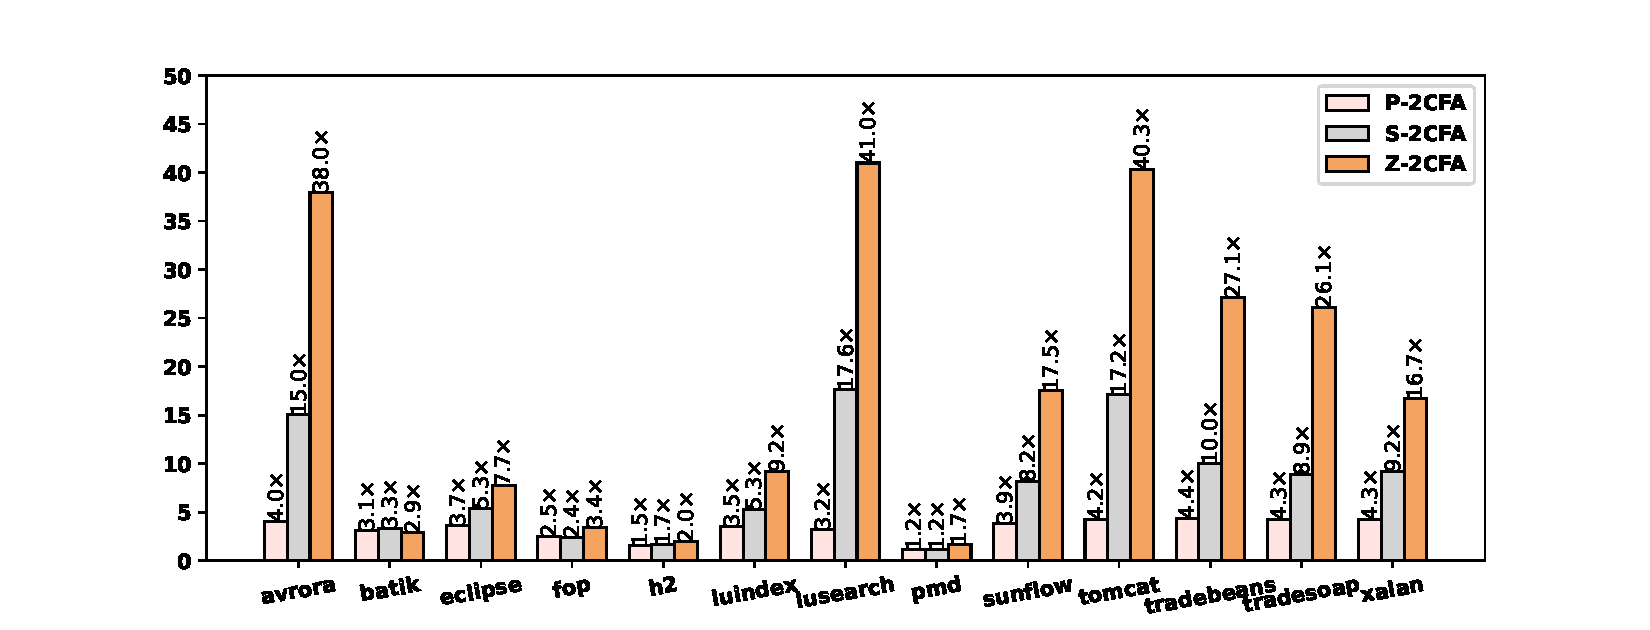
\includegraphics[width=\textwidth]{speedupktwo.pdf}
     \caption{$k=2$}
     \label{fig:twocfaspeedup}
\end{subfigure}
\begin{subfigure}[b]{\textwidth}
     \centering
     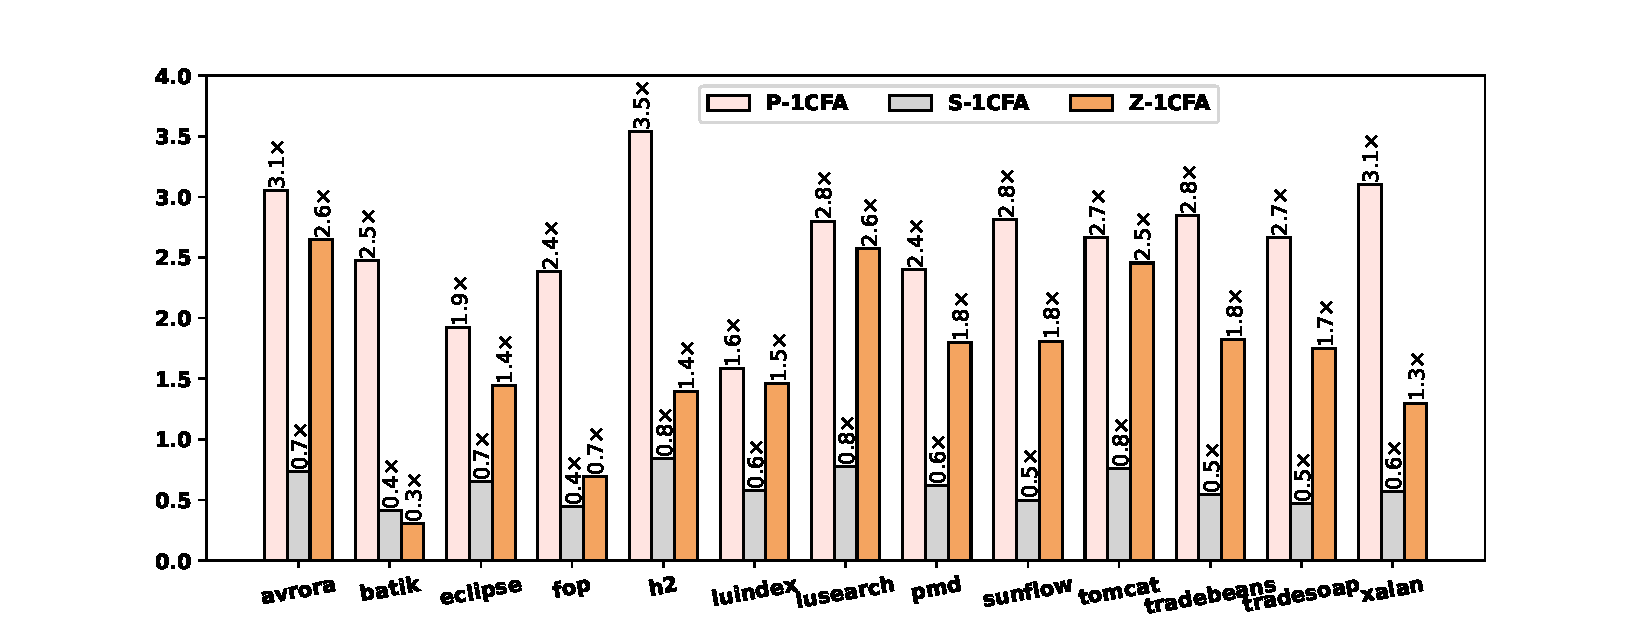
\includegraphics[width=\textwidth]{speedupkone.pdf}
     \caption{$k=1$}
     \label{fig:onecfaspeedup}
 \end{subfigure}
 \hfill
\caption{The speedups of \pkcs{k}, \skcs{k}, and \zkcs{k} over \kcs{k} based on the analysis times in \Cref{tab:main}.
%How the speedups are computed is explained precisely in \Cref{eqn:speedups}. 
}
\label{fig:speedups}
\end{figure}

\begin{comment}
\paragraph*{Effectiveness}
\label{subsec:effectiveness}

% \tooll is slightly slower than \spark but can analyze all the 12 programs in under 26s each.

% The overall overheads from \spark, \toolp, and \tooll is acceptable for two reasons: First, as $k$ increases, the overheads are negligible relative to the analysis time of \kcs{k}.   Second, these overheads can be amortized. The points-to information produced by \spark is often reused for some other purposes (e.g., constructing inter-procedural control
% flow graph \cite{flowdroid2014}), and the same pre-analysis performed by \toolp and \tooll can 
% be shared for accelerating a range of \kcs{k}-based pointer analysis algorithms (e.g., $k \in \{1, 2\}$ here.

\begin{table}[t]
\centering
%\vspace*{-1ex}
% \def\arraystretch{1.0}
\setlength{\tabcolsep}{1.2ex}
\caption{The analysis times of \spark and \tool in seconds. \label{tab:pretime}}
% \vspace*{-5.3ex}
\scalebox{0.92}{
\addtolength{\tabcolsep}{-0.54ex}
% \hspace{-2mm}
\small
\begin{tabular}{|c|l|r|r|r|r|r|r|r|r|r|r|r|r|}
	\hline
	   Prog.     & avrora & batik & eclipse &  fop &   h2 & luindex & lusearch &  pmd & sunflow & tomcat & tradebeans & tradesoap & xalan \\ \hline
	\textsc{Spark} & 6.6    &  31.2 &    14.6 & 74.7 & 16.3 &    20.6 &      5.2 & 20.1 &     9.8 &    7.3 &        8.4 &       8.1 &   8.6 \\ \hline
	    \tool      & 1.2    &   4.8 &     2.0 & 10.9 &  2.9 &     1.8 &      1.0 &  3.1 &     1.8 &    1.3 &        1.7 &       1.6 &   1.5 \\ \hline
\end{tabular}
	}
% 	\vspace*{-3.7ex}
\end{table}
\end{comment}


\begin{comment}
\begin{table}[htbp]
\centering
% \def\arraystretch{1.0}
\setlength{\tabcolsep}{1.2ex}
\caption{The analysis times of \spark and \tool in seconds. \label{tab:pretime}}
\scalebox{1}{
% \addtolength{\tabcolsep}{-0.6ex}
\hspace{-5mm}
\small
\begin{tabular}{|c|c|c|c|c|c|c|}
\hline
Prog. &antlr&bloat&chart&eclipse&fop&hsqldb\\
\hline
\textsc{Spark}&4.8&5.6&8.5&5.7&4.3&4.1\\
\hline
\tool &0.7&0.8&1.0&0.8&0.6&0.6\\
\hline
\hline
Program&lusearch&pmd&xalan&checkstyle&findbugs&JPC\\
\hline
\textsc{Spark}&3.9&7.6&4.6&8.0&9.1&7.7\\
\hline
\tool &0.5&0.9&0.7&1.0&1.0&0.9\\
\hline
\end{tabular}
	}
\end{table}
\end{comment}




\begin{comment}
According to \Cref{tab:pretime}, 
\tool is effective as a pre-analysis as it is lightweight (running in linear time of
the PAG edges in a program).
In terms of the average analysis time spent on analyzing
the 13 benchmarks, there are 
\sparkPreTime seconds for \spark but only 
 \toolPreTime seconds for \tool.
\end{comment}

 
% Note that the pre-analysis time of \tool for a program can be further amortized
 
%\tool is significantly faster than \spark as it is based on a linear selection algorithm.  On average, we have \toolPreTime seconds (\tool), ≈. 
% \Cref{tab:pretime} also includes the analysis time of \spark \cite{lhotak2003scaling} as the selection algorithms works on a subset of methods $\mathbb{M}$ that are reachable during the context-insensitive analysis.  $\mathbb{M}$ would be a superset of methods that are reachable during the context-sensitive analysis (e.g., \kcs{k}). \tooll also relies on \spark to pre-compute a set of monomorphic calls for its optimization.
% except \tool, \spark and our two optimizations, \toolp and \tooll, 
 

When considering both the precision and efficiency achieved  by \pkcs{k}, \skcs{k} and \zkcs{k}, we can draw several conclusions. First,  for precision-critical client analyses such as software security analysis,  \pkcs{k} is recommended since it not only runs significantly faster than the baseline \kcs{k} but also preserves its precision.
Second, for certain client analyses that expect to use a pointer analysis that has
the precision of \kcs{1} but runs as fast as possible, \pkcs{1} is recommended
as it is faster than \skcs{1} and \zkcs{1} while achieving the same precision as \kcs{1}. Finally, for certain client analyses that expect to use a pointer
analysis with the precision of \kcs{2},
our recommendation is \zkcs{2} if these clients prioritize efficiency over precision
(by trading willingly some loss of precision
for efficiency gains), or \skcs{2} if these clients still
prioritize efficiency over precision but can only accept a negligible  loss of
precision, or \pkcs{2} otherwise (i.e., if these
clients prioritize precision over efficiency but still expect the pointer
analysis to run as fast as possible).


\paragraph*{Discussion}
\label{subsec:threatstovalidity}

{
The analysis times of  \kcs{k}, \pkcs{k}, \skcs{k}, and \zkcs{k}, and consequently, the   speedups achieved by  \pkcs{k}, \skcs{k}, and \zkcs{k} over \kcs{k}, may  depend on the
 pointer analysis frameworks in which \kcs{k}, \pkcs{k}, \skcs{k}, and \zkcs{k} are implemented and
the  benchmarks selected during the evaluation.
In this work, we have conducted
our evaluation in a popular pointer analysis framework \soot by using all the
benchmarks (except \texttt{jython}) from the latest DaCapo benchmark suite and comparing \kcs{k}, \pkcs{k}, \skcs{k}, and \zkcs{k} under the same standard experimental setting used in the pointer analysis literature \cite{He2021Turner, tan2017efficient, li2018precision}. Our evaluation shows that \LFCR can
enable \pkcs{k} to  run faster than \kcs{k} without any precision loss.
In addition, our evaluation also shows 
that \pkcs{k} represents a new alternative to \skcs{k} and
\zkcs{k}, advancing the state of the art in accelerating \kcs{k} with
selective context-sensitivity.

